\section{RESULTS}
\label{sec:Res}

We prove the validity of the geometric hints in semantic surface segmentation and evaluate our method on two widely used dataset: Hedau's dataset \cite{hedau2009recovering} and LSUN dataset \cite{zhang2015large}. 

\subsection{Analysis of Geometric Hints}
\label{sec:ablation}
To explore the benefits of geometric hints for semantic surface segmentation, we train FCNs with or without geometric hints as additional input. Their performance are evaluated on LSUN validation set using pixel error of $\vb{\hat{L}}$, see Table~\ref{table:ablation}. To make fair comparisons with \cite{ren2016coarse, dasgupta2016delay}, both of which are built on VGG16, we train an MC-FCN based on VGG16 too. For \cite{ren2016coarse}, we directly apply their trained model to generate $\vb{\hat{L}}$. And for \cite{dasgupta2016delay}, we train an FCN having the same architecture in \cite{dasgupta2016delay}. As revealed by Table~\ref{table:ablation}, with the help of geometric hints, our MC-FCN obtain lower pixel error of $\vb{\hat{L}}$. We further improve the performance by employing a ResNet101 based FCN. Qualitative results are demonstrated in Fig.~\ref{fig:fcn-comparison}. (a)-(e) show typical good examples. Intuitively, the geometric hints help remove the spurious regions caused by clutter and generate more accurate semantic surface segmentation. (f) depicts a generally bad case that FCNs tend to be cheated by large truncated wall-like object surface, e.g., the bed looks like the floor. (g) is an another kind of bad case led by clutter while our MC-FCN seems to produce relatively clear results.  

\begin{figure}[!ht]
	\centering 
	\textsc{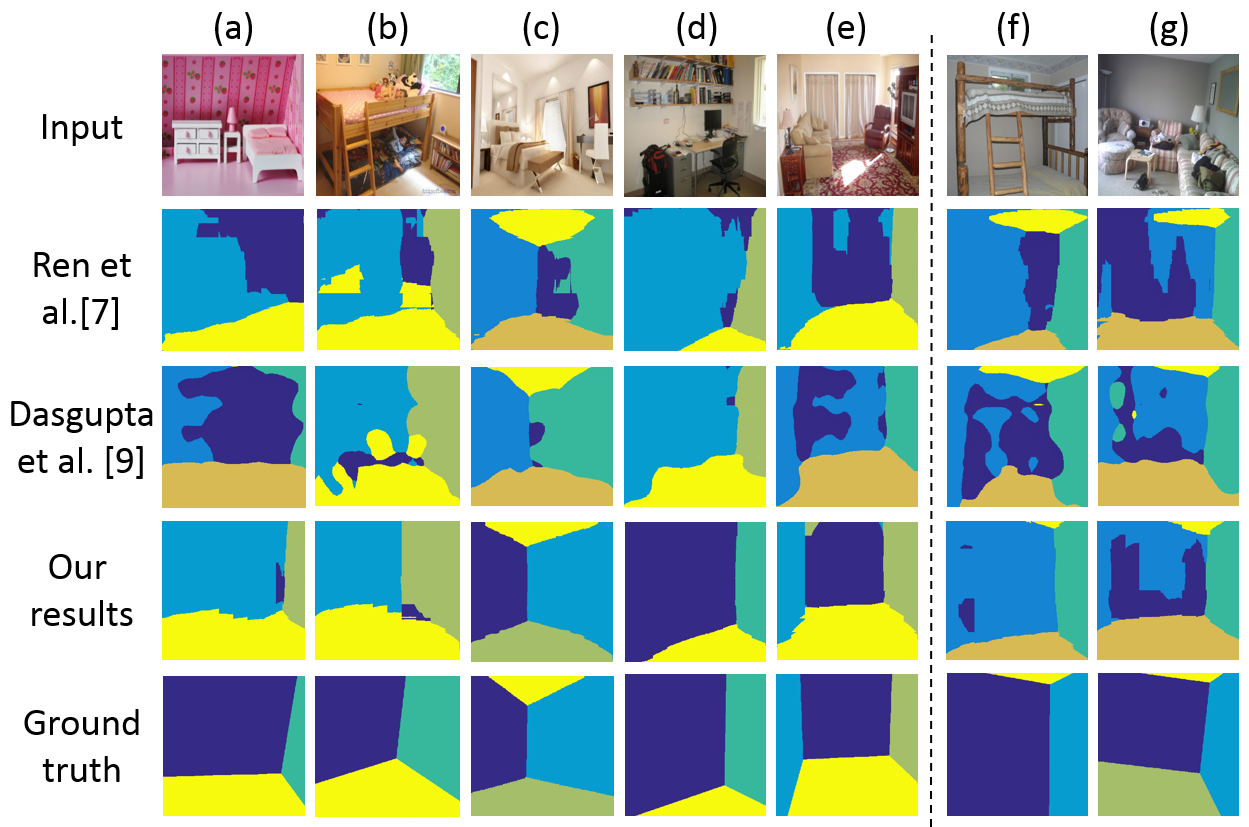
\includegraphics[width=8.5cm]{figure/compare1.png}}
	\caption{Surface segmentation results using different architectures. All the networks are built on VGG16 architecture. Our MC-FCN with geometric hints generates more robust segmentation facing complex environmental factors.}
	\label{fig:fcn-comparison}
\end{figure}

\begin{table}
	\centering
	\begin{tabular}{lc}
		\toprule
		Network & $\epsilon_{pixel}$ (\%)\\
		\midrule
		Ren et al.~\cite{ren2016coarse} & 21.54 \\
		Dasgupta et al.~\cite{dasgupta2016delay} & 15.86 \\  
		\midrule
		MC-FCN (VGG16)  & 14.05 \\
		MC-FCN (ResNet101) & 12.41 \\
		\bottomrule
	\end{tabular}
	\caption{Pixel error of semantic surface segmentation by different FCNs. By utilizing geometric hints, our proposed MC-FCN acquire more accurate segmentation. }	
	\label{table:ablation}
\end{table}

\subsection{LSUN Results}
\label{sec:LSUN}
We train our multi-channel FCN on the relabeled LSUN dataset released by \cite{ren2016coarse}. The dataset consists of 4000 training, 394 validation, and 1000 testing images. We extract geometric hints from original images and resize all the images, depth and normal maps to $321\times321$ using bicubic interpolation. Then these three types of data are integrated to train the ResNet101 based multi-channel FCN. We evaluate our results using the official toolkit which provides two standard metrics: pixelwise error and corner error. The pixelwise error is computed by counting the percentage of pixels that are mismatched. (The Hungarian algorithm is applied to address the labeling ambiguity problem) The corner error is computed by calculating the Euclidean distance between predicted corners and corresponding ground truth corners.

Our performance on LSUN test set compared with other methods is shown in Table~\ref{table:comparison-lsun}. Qualitative results are displayed in Fig.~\ref{fig:qualitative}. Our approach outperforms conventional methods \cite{hedau2009recovering,mallya2015learning} and most neural network based methods  \cite{zhang2017learning,dasgupta2016delay,ren2016coarse,LeeRoomNet17}. 
%
Besides, when training the FCN, Zhao et al.~\cite{zhao2017physics} formulate the room layout using boundaries among semantic surfaces, while we formulate the room layout using the five semantic surfaces as \cite{dasgupta2016delay} do. These two representation may have different application prospects in the future. For example, when a home robot wants to locate itself while moving, the semantic boundaries are not always available. Our method may also be an inspiration for other surface estimation problems.

\comments{
This kind of boundary representation has a intrinsic problem of unbalanced training data where most of the area is background. This may be the reason for the training problem, as claimed in \cite{zhao2017physics,mallya2015learning}. They both have to pretrain their model on an indoor scene dataset to make the training stable. While we formulate the room layout using the five semantic surfaces as \cite{dasgupta2016delay} do, our representation does not have this limitation. We pretrain our MC-FCN on both indoor scene dataset (SUNRGBD) and non-indoor scene dataset (PASCAL) separately. Both settings lead to stable training and competitive performance, as shown in \ref{table:comparison-lsun}. The model pretrained on SUNRGBD obtains a better result which should benefit from external indoor scene data in SUNRGBD. }


\comments{
This boundary representation and its variants are adopted in \cite{zhang2017learning,ren2016coarse}, while we formulate the room layout using the five semantic surfaces as \cite{dasgupta2016delay} do. 
%
Which formulation is better for room layout estimation remains an open question, especially when the room can not be exactly modeled as a cube due to special architectural structures such as slope roof, pillar and condole top. Boundary representation may be less robust to these situations and LSUN dataset contains few of these cases. Moreover, the two representation may work togehter to improve both performance in a joint training way, which is possible claimed by \cite{mallya2015learning,ren2016coarse}.}


\begin{figure}[!ht]
	\centering
	\textsc{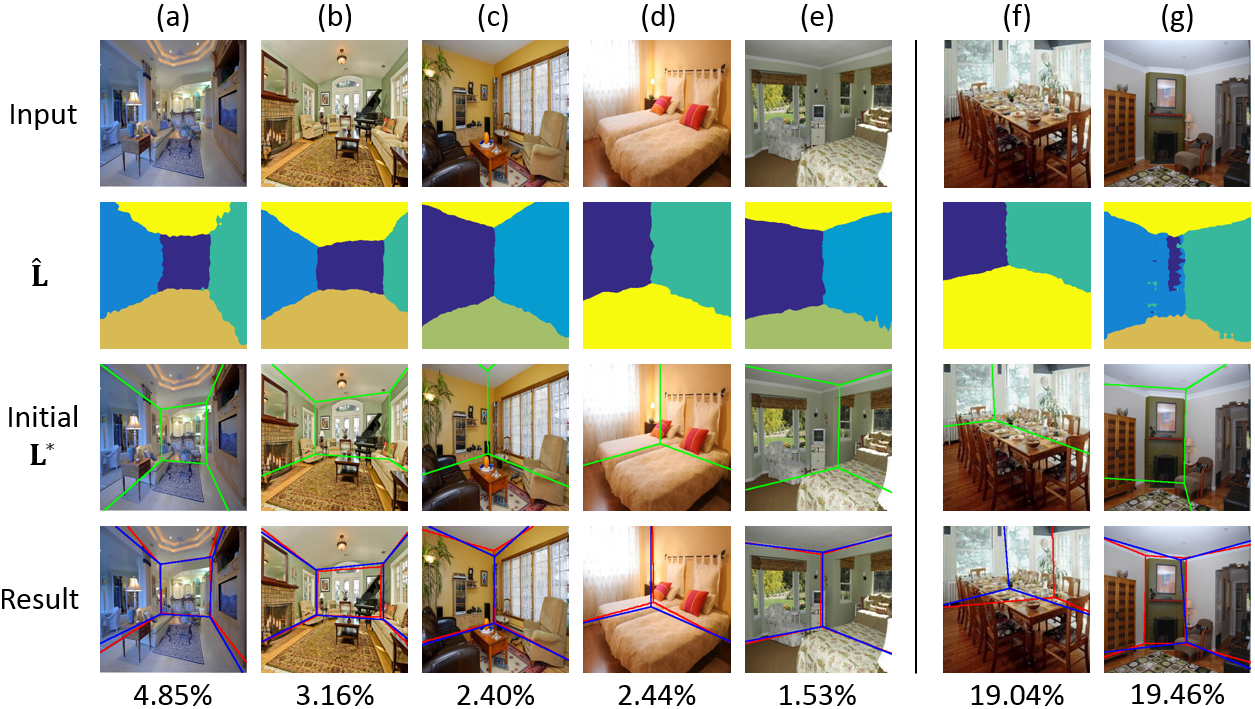
\includegraphics[width=8.5cm]{figure/qualitive.png}}
	\caption{Qualitative results of our methods on LSUN validation set. (a)-(e) depict precise results. (f)(g) show failure cases misled by $\vb{\hat{L}}$. }
	\label{fig:qualitative}
\end{figure}

\begin{table}
	\centering 
	\begin{tabular}{lcc}
		\toprule
		Method & $\epsilon_{corner}$ (\%) & $\epsilon_{pixel}$ (\%) \\
		\midrule
		Hedau et al.~\cite{hedau2009recovering} & 15.48 & 24.23 \\
		Mallya et al.~\cite{mallya2015learning} & 11.02 & 16.71 \\
		Zhang et al.~\cite{zhang2017learning} & 8.70 & 12.49 \\
		Dasgupta et al.~\cite{dasgupta2016delay} & 8.20 & 10.63 \\
		Ren et al.~\cite{ren2016coarse} & 7.95 & 9.31 \\
		Lee et al.~\cite{LeeRoomNet17} & 6.30 & 9.86 \\
		Zhao et al.~\cite{zhao2017physics} & 3.84 & 5.29 \\
		\midrule
		Proposed MC-FCN & 6.26 & 8.61 \\
		\bottomrule
	\end{tabular}
	\caption{Performance on the LSUN~\cite{zhang2015large} dataset}	
	\label{table:comparison-lsun}
\end{table}

\subsection{Hedau Results}
\label{sec:Hedau}
We also conduct experiment on a relatively smaller dataset published by \cite{hedau2009recovering}, which consists of 209 training images and 104 testing images. We follow the experimental setup in \cite{LeeRoomNet17} and directly predict the semantic surface on Hedau's test set using the model trained on LSUN. Pixel error is adopted to evaluate the final results, see Table~\ref{table:comparison-hedau}. Our performance is better than \cite{mallya2015learning,zhang2017learning,ren2016coarse}, all of which have trained their model on Hedau's training set. This indicates that our model has a good generalization ability. We achieve the performance close to state-of-the-art on this dataset.

\begin{table}
	\centering 
	\begin{tabular}{lc}
		\toprule
		Method & $\epsilon_{pixel}$ (\%) \\
		\midrule
		Hedau et al.~\cite{hedau2009recovering} & 21.20 \\
		Mallya et al.~\cite{mallya2015learning} & 12.83 \\
		Zhang et al.~\cite{zhang2017learning} & 12.70 \\
		Dasgupta et al.~\cite{dasgupta2016delay} & 9.73 \\
		Ren et al.~\cite{ren2016coarse} & 8.67 \\
		Lee et al.~\cite{LeeRoomNet17} & 8.36 \\
		Zhao et al.~\cite{zhao2017physics} & 6.60 \\
		\midrule
		Proposed MC-FCN & 6.63 \\
		\bottomrule
	\end{tabular}
	\caption{Performance on the Hedau's~\cite{hedau2009recovering} dataset}
	\label{table:comparison-hedau}
\end{table}



